\documentclass[11pt, a4paper]{article}	% Alternativet er å bruke {report}, men vi holder oss helst til {article} i labrapportene
\usepackage[utf8]{inputenc}
\usepackage[T1]{fontenc} 								% Vise norske tegn

\usepackage{graphicx} 
      						% For å inkludere figurer
%\setcounter{secnumdepth}{0} 						% \section nummereres ikke

% Justeringer av defaultverdier for teksten på siden:
\setlength{\textheight}{240mm} 
\setlength{\textwidth}{150mm}  
\topmargin -5mm 
\oddsidemargin -5mm


%%%%%%%%%%%%%%%%%%%%%%%%%%%%%%%%%%%%%%%%%%%%%%%%%%%%%%%%%%%%%%%%%%%%%%%%%
\begin{document}

\begin{titlepage}
\newcommand{\HRule}{\rule{\linewidth}{0.5mm}}
 
\begin{center}
 

\textsc{\huge TDT4190 }\\[2.0cm]

 
\HRule \\[0.3cm]
{\huge \bfseries  Øving  1
\\\ \\\ \LARGE Kjetil Sletten, Simen Skoglund og Christian Peter }\\[0.4cm]
\HRule \\[1.5cm]
 
\vfill
 
{\large \today}
 
\end{center}
\end{titlepage}

\section{Kort beskrivelse}
Vi har valgt å lage en egen klasse som implementer Java RMI. Hver klasse er beskrevet nedenfor. Her er et overblikk over det som skjer:
\begin{center}
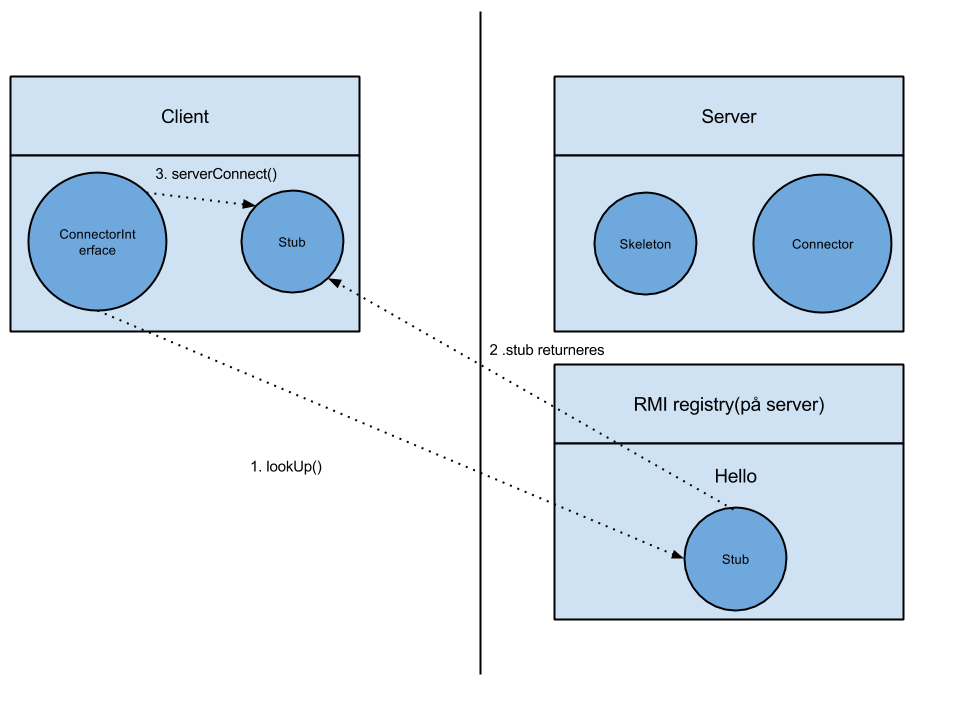
\includegraphics[scale=0.5]{TicTacToe}
\end{center}

Klienten må ha tak i stub-objektet, for å få tak i dette må klienten da gjøre et lookup. Siden RMI registry allerede har laget stuben som klienten leter etter, trenger klienten bare å spørre om denne stubben finnes. Deretter vil RMI reqgistry returnere stubben, som klienten da vil snakke sammen ved å overføre de metodene som er blitt definert i interfacet. 


\section{Connector.java}
\subsection*{public void serverConnect()}
Denne koden vil bli kjørt hvis det ikke finnes noen server. Da vil isServer bli satt til true slik at vi kan bruke dette til å bestemme hvilket merke den skal bruke. Vi benytter oss av Registry der vi åpner det på port 3050 for øyeblikket.
\subsection*{public ConnectorInterface clientConnect()}
Hvis det ikke går ann å sette opp en server, vil clientConnect kjøres. Denne metoden vil enten retunere servers grensesnittet eller klient grensesnittet slik at klassen TicTacToe.java kan bruke denne.


\subsection*{public boolean setMark(int x, int y, char mark)}
Metode for å sette merke(O eller X) på motstanderens skjerm.
\subsection*{public boolean serverTurn(boolean server)}
Denne metoden setter om det er serveren sin tur til å spille.
\subsection*{public boolean isServer()}
En enkel metode for å se om man selv er server eller klient.
\subsection*{public void setOpponent(ConnectorInterface opponent)}
Når klienten har koblet seg opp, er det ikke noen automatikk i at serveren vet hvem denne klienten er. Derfor lagde vi denne metoden som setter motstanderen for serveren så den kan sende merker tilbake til klienten når det spilles.
\subsection*{public void setGameIsWon(boolean gameIsWon)}
For å hindre at det skal kunne spilles videre når en har vunnet må man si ifra til motstanderen at man har vunnet. Dette gjør denne metoden.

\subsection*{public void resetGame(int boardSize) }
Dette er en ekstra funksjonalitet som vi har lagt til. Det vi gjør her er å starte spillet på nytt på både server og klient.

\section{ConnectorInterface.java}
Grunnen til at vi har med denne er at vi trenger et interface som kan brukes av klienten på den andre siden. Dette grensesnittet implementerer Remote. Metodene som ligger her er beskrevet i Connector.java seksjonen.

\section{BoardModel.java}
\subsection*{public void cleanBoard()}
Denne metoden måtte jeg legge til for å fjerne alle kryss og sirkler. Ingenting som har med RMI er gjort her.

\section{TicTacToe.java}



\end{document}